In questa capitolo si descriverà il problema affrontato per poi passare alle versioni sequenziale e distribuita della soluzione (è possibile trovare le due versioni sulla piattaforma di versioning GitHub), e infine si discuterà delle prestazioni delle due versioni.
\section{Descrizione del problema}
Il problema affrontato in questo studio riguarda l'applicazione dell'algoritmo \textbf{SIFT}(Scale-Invariant Feature Transform) per effettuare object detection. L' object detection è una tecnologia informatica correlata alla visione artificiale e all'elaborazione di immagini che si occupa di rilevare istanze di oggetti semantici di una determinata classe in immagini e video digitali. Il rilevamento di oggetti ha applicazioni in molte aree della visione artificiale, tra cui il recupero di immagini e la videosorveglianza. Per ogni oggetto in un'immagine, ci sono molte features, che sono caratteristiche interessanti dell'oggetto, le quali possono essere estratte in modo da fornire una descrizione "caratteristica" dell'oggetto. Questa descrizione estratta da un'immagine campione può poi essere utilizzata per identificare l'oggetto durante il tentativo di individuare l'oggetto in un'immagine contenente più oggetti. Per poter recuperare queste features esistono diversi algoritmi quali per esempio \textbf{SURF}(Speeded Up Robust Features), \textbf{ORB} (Oriented FAST and Rotated BRIEF) e \textbf{SIFT}. In questo studio ci siamo concentrati su quest'ultimo il quale è un algoritmo cpu-intensive e quindi ci interessava analizzare il suo comportamento in un ambiente distribuito.
\subsection{SIFT}
Scale-invariant feature transform (SIFT) è un algoritmo utilizzato in computer vision che permette di rilevare e descrivere caratteristiche pubblicato da David G. Lowe\cite{lowe04} nel 2004. L'algoritmo consiste in un metodo in grado di estrarre delle caratteristiche distintive invarianti da un'immagine che possono essere utilizzate per effettuare un matching tra diversi oggetti. Le caratteristiche sono invarianti rispetto alla scala e alla rotazione dell'immagine e sono mostrate per fornire una robusta corrispondenza su una vasta gamma di distorsioni affini, cambiamenti nel punto di vista 3D, aggiunta di rumore e cambiamento nell'illuminazione. L'algoritmo esegue cinque step:
\begin{itemize}
\item \textbf{Scale-space Extrema Detection}
Per poter individuare dei keypoints abbiamo bisogno di diverse scale di un immagine quindi viene applicato un filtro per la scala. Questo filtro utilizza la \textbf{Laplaciana di una Gaussiana}(LoG) che permette di rilevare blob di varie dimensioni grazie all'utilizzo di $\sigma$ che funge come parametro di scala. Poichè LoG è costoso SIFT usa la differenza gaussiana(DoG) come alternativa che è una approssimazione del primo. La DoG è ottenuta come differenza di sfocatura gaussiana di un immagine con diversi $\sigma$ (si parte da un valore iniziale di $\sigma$ fino ad arrivare $k\sigma$) . Questo processo viene eseguito per diverse ottave dell'immagine.
\begin{figure}[ht]
	\begin{center}
    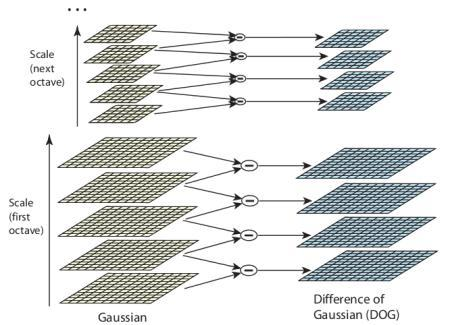
\includegraphics[scale=0.7]{DoG.jpg}
    \caption{Ottave di un immagine}
    \label{fig:DoG}
    	\end{center}
\end{figure}
Una volta trovato DoG vengono cercati i keypoints che rappresentano meglio l'immagine confrontando i pixel su diverse scale, per esempio un pixel in una immagine viene confrontato con i suoi 8 vicini e e con i 9 pixel della scala precedente e successiva.
\begin{figure}[ht]
  \begin{center}
    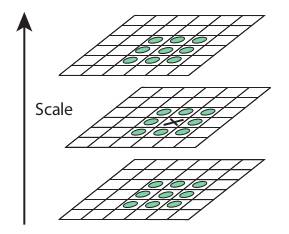
\includegraphics[scale=0.7]{kp.jpg}
    \caption{Ricerca di un keypoints}
    \label{fig:kp}
    	\end{center}
\end{figure}
Il paper fornisce alcuni dati ottimali e sono: numero di ottave = 4, livelli di scala = 5 valore iniziale $\sigma$ = 1.6 e k = $\sqrt{2}$.
\item \textbf{Keypoint Localization}
Una volta individuati potenziali keypoints, devono essere affinati per ottenere risultati più accurati. Viene usata l'espansione della serie di Taylor dello spazio di scala per ottenere una posizione più accurata dei punti e, se l'intensità di un punto è inferiore a un valore di threshold (0,03 valore di soglia del paper), viene rifiutata.
La DoG(Difference of Gaussian) ha una risposta più alta per gli edge e che quindi vanno rimossi, per fare questo SIFT usa una matrice Hessiana 2x2 per computare la curvatura per poi confrontarla con la threshold degli edge se viene superata allora gli edge vengono rimossi
\item \textbf{Orientation Assignment}
Successivamente viene assegnato un orientamento a ciascun keypoint per ottenere l'invarianza alla rotazione dell'immagine. Dei vicini vengono presi attorno alla posizione del punto in base alla scala, e al modulo del gradiente e la direzione vengono calcolate in quella regione. Viene creato un istogramma di orientamento con 36 contenitori a 360 gradi. Viene pesato per il modulo del gradiente e la gaussian-weighted circular window con $\sigma$ uguale a 1,5 volte la scala del punto chiave, viene preso il picco più alto nell'istogramma e anche qualsiasi picco superiore a 80 vengono considerati per calcolare l'orientamento.
\item \textbf{Keypoint Descriptor}
In questa fase viene creato un descrittore di keypoint. Viene preso un intorno 16x16 attorno al keypoint. Viene  diviso in 16 sotto blocchi di dimensione 4x4. Per ciascun sottoblocco viene creato un istogramma di orientamento a 8 bin. Quindi sono disponibili in totale 128 valori bin. Questo rappresentato come un vettore per formare un descrittore di keypoints. Oltre a questo, vengono prese diverse misure per ottenere robustezza contro i cambiamenti di illuminazione, la rotazione ecc.
\item \textbf{Keypoint Matching}
I keypoints tra due immagini sono abbinati identificando i loro vicini più vicini. Ma in alcuni casi, la seconda corrispondenza più vicina potrebbe essere molto vicina alla prima. Questo può accadere a causa di rumore o per altri motivi. In questi casi, viene preso il rapporto tra distanza più vicina e distanza più vicina al secondo. Se è maggiore di 0.8, vengono rifiutati. In questo modo si riesco a eliminare circa il 90\% di false corrispondenze mentre scarta solo il 5\% corrispondenze corrette.
\end{itemize}
\subsection{OpenCV}
Per l'implementazione dell'object detection è stato utilizzato OpenCV. OpenCV (Open Source Computer Vision Library) è una libreria open source di computer vision e di apprendimento automatico, realizzato per fornire un'infrastruttura comune per le applicazioni di visione artificiale e per accelerare l'uso della percezione della macchina nei prodotti commerciali. OpencCV è rilasciato con licenza BSD e la sua libreria ha più di 2500 algoritmi ottimizzati, che comprendono un set completo di algoritmi di visione artificiale e di apprendimento automatico sia classici che all'avanguardia. questi algoritmi possono essere utilizzati per rilevare e riconoscere i volti, identificare gli oggetti, classificare azioni umane nei video, tracciare i movimenti della telecamera, tracciare oggetti in movimento, estrarre modelli 3D di oggetti, trova immagini simili da un database di immagini, rimuovi gli occhi rossi dalle immagini scattate con il flash, segui i movimenti degli occhi, riconosci i paesaggi e stabilisci i marcatori per sovrapporli alla realtà aumentata, ecc. OpenCV supporta diversi linguaggi C++, Python, Java e MATLAB e i pricipali sistemi operativi Linux, Windows Mac os, e Android.
\section{Versione Sequenziale}
Il core della versione sequenziale è il \emph{\textit{SiftManager}}. L'algoritmo prevede l'individuazione di un unico oggetto(query) all'interno di una o più scene(train). Il nostro algoritmo esegue cinque step:
\begin{itemize}
\item \textbf{Fase Uno :}\\
Vengono estratte le caratteristiche grazie all'algoritmo SIFT dall'immagine query e dall'immagine di train.
Prima vengono estratti i keypoints attraverso \emph{\textit{extractKeypoints}} e successivamente i descrittori con \emph{\textit{extractDescriptors}}
\begin{lstlisting}
 public static MatOfKeyPoint extractKeypoints(Mat image, Feature2D extractor) {
    MatOfKeyPoint imageKeypoint = new MatOfKeyPoint();
    extractor.detect(image, imageKeypoint);
    return imageKeypoint;
  }

  public static MatOfKeyPoint extractDescriptors(Mat image, MatOfKeyPoint imageKeypoints, Feature2D extractor) {
    MatOfKeyPoint imageDescriptors = new MatOfKeyPoint();
    extractor.compute(image, imageKeypoints, imageDescriptors);
    return imageDescriptors;
  }
\end{lstlisting}
\item \textbf{Fase Due :}\\
Viene effettuato il match tra le immagini query e train utilizzando l'algoritmo di Brute Force e utilizzando knnMatch con k = 2 , dove k indica il conteggio delle migliori corrispondenze trovate per ogni descrittore di query , inoltre viene effettuato anche il \textbf{ratio test} di Lowe (il valore ottimale per il ratio test è 0.75, dal paper di Lowe) sulle distanze dei punti per ogni coppia di match trovato, in modo da filtrare dei possibili falsi positivi.
\begin{lstlisting}
  public static MatOfDMatch calculateMatches(MatOfKeyPoint objectDescriptor, MatOfKeyPoint sceneDescriptor, DescriptorMatcher matcher) {
    List<MatOfDMatch> knnMatches = new ArrayList<>();
    matcher.knnMatch(objectDescriptor, sceneDescriptor, knnMatches, 2);
    List<DMatch> listOfGoodMatches = new ArrayList<>();
    for (int i = 0; i < knnMatches.size(); i++) {
      if (knnMatches.get(i).rows() > 1) {
        DMatch[] matches = knnMatches.get(i).toArray();
        if (matches[0].distance < RATIO_THRESHOLD * matches[1].distance) {
          listOfGoodMatches.add(matches[0]);
        }
      }
    }
    MatOfDMatch goodMatches = new MatOfDMatch();
    goodMatches.fromList(listOfGoodMatches);
    return goodMatches;
}
\end{lstlisting}
\item \textbf{Fase Tre :}\\
Viene rilevato l'oggetto tracciandone calcolandone l'omografia.
\begin{lstlisting}
  public static Mat localizeObject(List<KeyPoint> objectKeypoints, List<KeyPoint> sceneKeypoints, MatOfDMatch goodMatches) {
    List<Point> obj = new ArrayList<>();
    List<Point> scene = new ArrayList<>();
    List<DMatch> listOfGoodMatches = goodMatches.toList();
    for (int i = 0; i < listOfGoodMatches.size(); i++) {
      obj.add(objectKeypoints
          .get(listOfGoodMatches.get(i).queryIdx).pt);
      scene.add(sceneKeypoints
          .get(listOfGoodMatches.get(i).trainIdx).pt);
    }
    MatOfPoint2f objMat = new MatOfPoint2f(), sceneMat = new MatOfPoint2f();
    objMat.fromList(obj);
    sceneMat.fromList(scene);
    Mat H = Calib3d.findHomography(objMat, sceneMat, Calib3d.RANSAC, RANSAC_THRESHOLD);
    return H;
}
\end{lstlisting}
\item \textbf{Fase Quattro:}\\
Si effettua una stima sulla bontà dell'omografia.
\begin{lstlisting}
  public static boolean checkHomography(Mat homography){
    double firstCheck = Math.abs(Math.abs(homography.get(0, 0)[0]) - Math.abs(homography.get(1, 1)[0]));
    double secondCheck = Math.abs(Math.abs(homography.get(0, 1)[0]) - Math.abs(homography.get(1, 0)[0]));
    return firstCheck <= 0.1 && secondCheck <= 0.1;
  }
\end{lstlisting}
\item \textbf{Fase Cinque:}\\
Se la stima avviene con successo si disegna l'immagine in output, mostrando i match e l'omografia.
\begin{lstlisting}
  public static Mat drawImage(Mat objectImage, Mat sceneImage, MatOfKeyPoint objectKeypoints, MatOfKeyPoint sceneKeypoints, MatOfDMatch matches, Mat homography) {
    Mat outputImage = new Mat();
    Features2d.drawMatches(objectImage, objectKeypoints, sceneImage, sceneKeypoints, matches, outputImage, Scalar.all(-1),
            Scalar.all(-1), new MatOfByte(), Features2d.NOT_DRAW_SINGLE_POINTS);
    Mat objCorners = new Mat(4, 1, CvType.CV_32FC2), sceneCorners = new Mat();
    float[] objCornersData = new float[(int) (objCorners.total() * objCorners.channels())];
    objCorners.get(0, 0, objCornersData);
    objCornersData[0] = 0;
    objCornersData[1] = 0;
    objCornersData[2] = objectImage.cols();
    objCornersData[3] = 0;
    objCornersData[4] = objectImage.cols();
    objCornersData[5] = objectImage.rows();
    objCornersData[6] = 0;
    objCornersData[7] = objectImage.rows();
    objCorners.put(0, 0, objCornersData);
    Core.perspectiveTransform(objCorners, sceneCorners, homography);
    float[] sceneCornersData = new float[(int) (sceneCorners.total() * sceneCorners.channels())];
    sceneCorners.get(0, 0, sceneCornersData);
    Imgproc.line(outputImage, new Point(sceneCornersData[0] + objectImage.cols(), sceneCornersData[1]),
            new Point(sceneCornersData[2] + objectImage.cols(), sceneCornersData[3]), RECT_SCALAR, 4);
    Imgproc.line(outputImage, new Point(sceneCornersData[2] + objectImage.cols(), sceneCornersData[3]),
            new Point(sceneCornersData[4] + objectImage.cols(), sceneCornersData[5]), RECT_SCALAR, 4);
    Imgproc.line(outputImage, new Point(sceneCornersData[4] + objectImage.cols(), sceneCornersData[5]),
            new Point(sceneCornersData[6] + objectImage.cols(), sceneCornersData[7]), RECT_SCALAR, 4);
    Imgproc.line(outputImage, new Point(sceneCornersData[6] + objectImage.cols(), sceneCornersData[7]),
            new Point(sceneCornersData[0] + objectImage.cols(), sceneCornersData[1]), RECT_SCALAR, 4);
    return outputImage;
}
\end{lstlisting}

\begin{figure}[ht]
  \begin{center}
    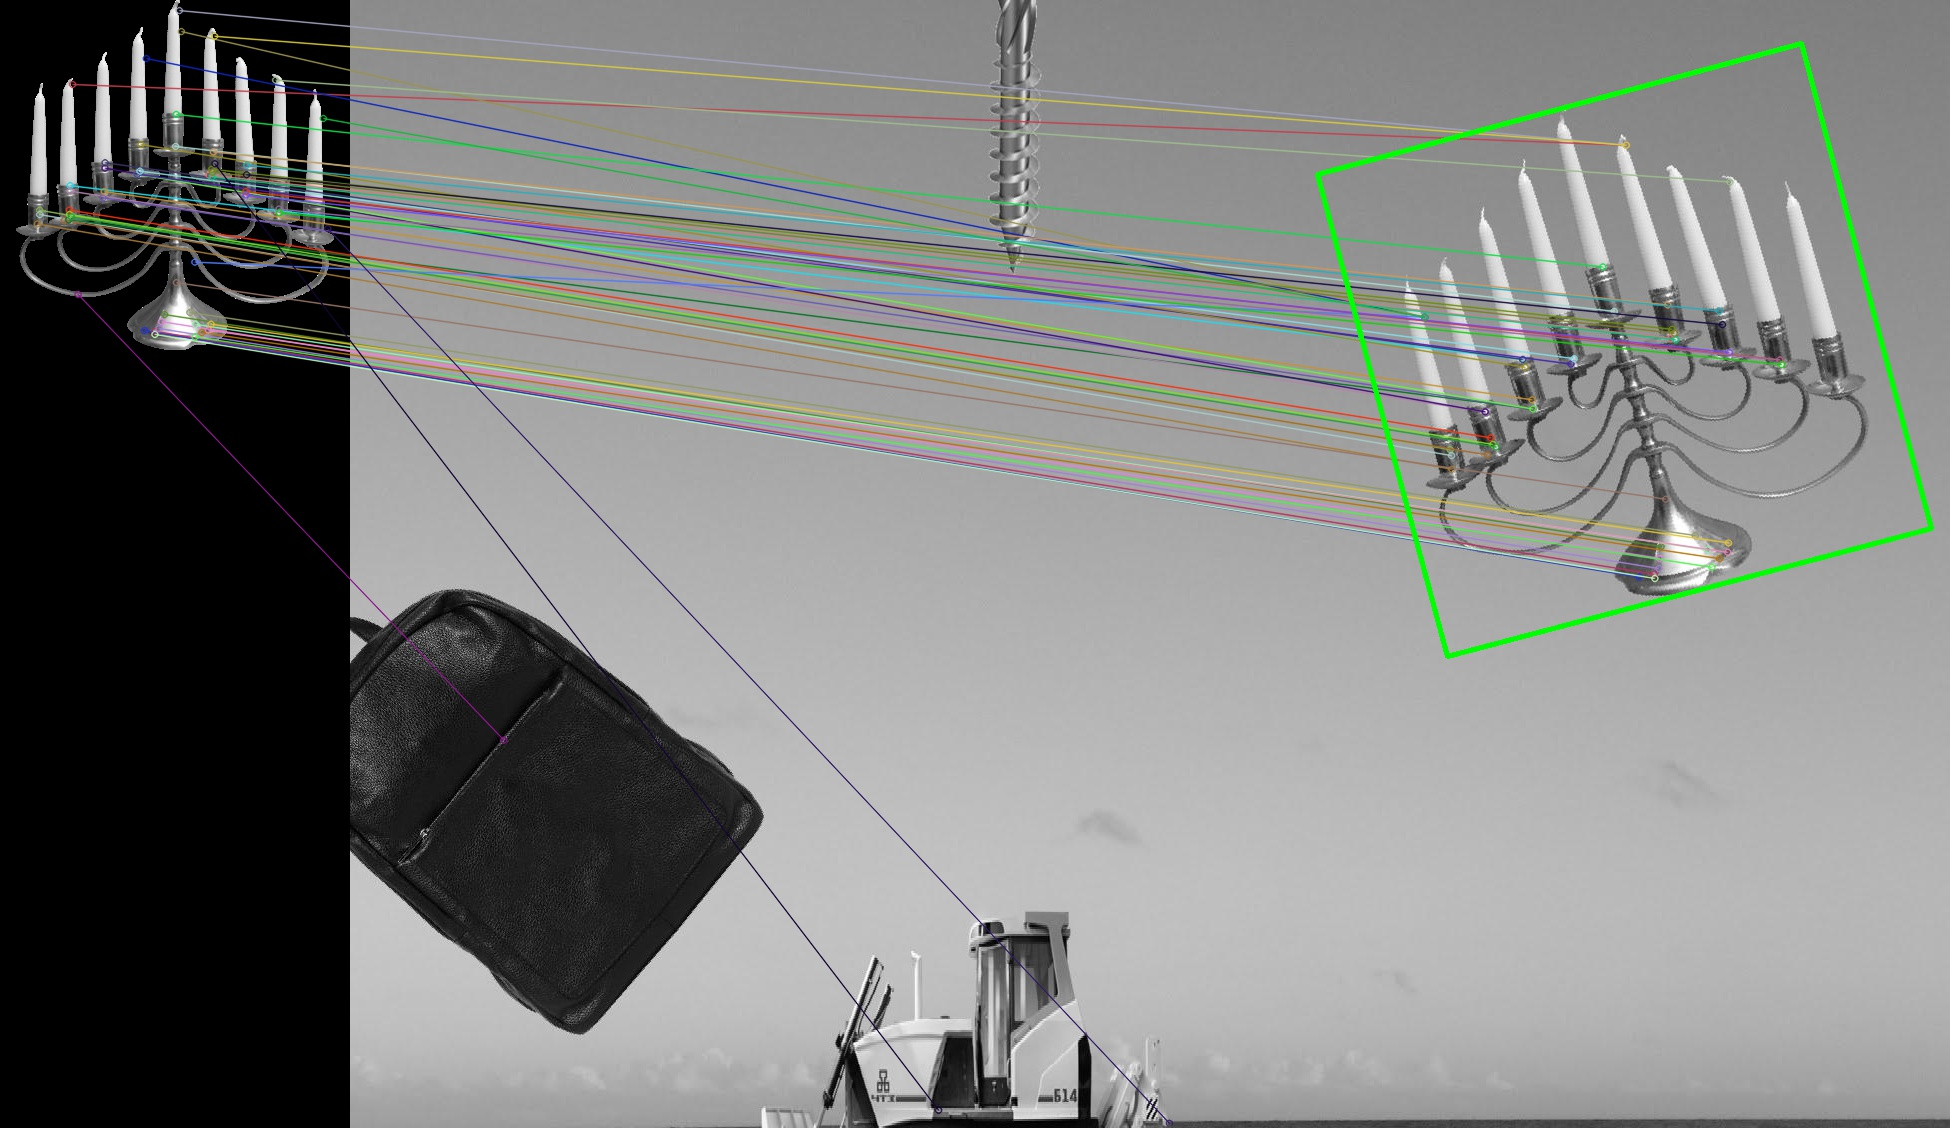
\includegraphics[width=\linewidth]{omografia.jpg}
    \caption{Esempio di esito positivo}
    \label{fig:hom}
    	\end{center}
\end{figure}

\end{itemize}.
\section{Versione Distibuita con Hadoop}
La versione distribuita funziona nel seguente modo, prese una serie di immagini query(oggetto da cercare) e una serie di train(scene) ogni oggetto viene cercato in tutte le scene.
Il core resta lo stesso visto precedentemente in \emph{\textit{SiftManager}} viene aggiunto  \emph{\textit{SiftUtilis}} che presenta delle funzioni di supporto per le diverse conversione necessarie per poter effettuare il trasferimento di immagini su Hadoop, \emph{\textit{SiftReduce}} per il reduce sul cluster di Hadoop, \emph{\textit{SiftMapper}} per il mapping ,\emph{\textit{MatWritable}} e \emph{\textit{MatOfKeyPointWritable}} per serializzare il risultato ottenuto dal reduce e poterlo passare al map.\\
\begin{itemize}

\item \textbf{Map}:\\
Il Map si occupa di estrarre i descrittori nei diversi oggetti da cercare successivamente nelle scene
\begin{lstlisting}
 @Override
  protected void map(Text key, MatWritable value, Context context) throws IOException, InterruptedException {
    SIFT sift = SIFT.create();
    SiftManager manager = SiftManager.getInstance();
    MatOfKeyPoint objectKeyPoints = manager.extractKeypoints(value.getImage(), sift);
    MatOfKeyPoint objectDescriptors = manager.extractDescriptors(value.getImage(), objectKeyPoints, sift);
    MapWritable map = new MapWritable();
    map.put(new Text(SiftUtils.OBJ_IMG), value);
    map.put(new Text(SiftUtils.OBJ_KPS), new MatOfKeyPointWritable(objectKeyPoints));
    map.put(new Text(SiftUtils.OBJ_DSC), new MatOfKeyPointWritable(objectDescriptors));
    context.write(key, map);
}
\end{lstlisting}

\item \textbf{Reduce}: \\
Il Reduce ha il compito di estrarre i descrittori della scena e successivamente di effettuare il match tra l'oggetto e la scena 
\begin{lstlisting}
protected void reduce(Text key, Iterable<MapWritable> values, Context context) throws IOException, InterruptedException {
    for (MapWritable map : values) {
      MatWritable receivedImage = ((MatWritable) map.get(new Text(SiftUtils.OBJ_IMG)));
      MatOfKeyPointWritable receivedKeyPoints = ((MatOfKeyPointWritable) map.get(new Text(SiftUtils.OBJ_KPS)));
      MatOfKeyPointWritable receivedObjectDescriptors = ((MatOfKeyPointWritable) map.get(new Text(SiftUtils.OBJ_DSC)));
      MatOfKeyPoint objectDescriptors = receivedObjectDescriptors.getMatOfKeyPoint();
      MatOfKeyPoint objectKeypoints = receivedKeyPoints.getMatOfKeyPoint();
      SiftManager manager = SiftManager.getInstance();
      FileSystem fs = FileSystem.get(context.getConfiguration());
      Path scenePath = Path.mergePaths(fs.getHomeDirectory(), new Path("/scenes"));
      RemoteIterator iterator = fs.listLocatedStatus(scenePath);
      SIFT sift = SIFT.create();
      while (iterator.hasNext()) {
        LocatedFileStatus lfs = (LocatedFileStatus) iterator.next();
        String format = SiftUtils.extractFormat(lfs.getPath().getName());
        String name = lfs.getPath().getName();
        if (lfs.isFile()) {
          InputStream input = fs.open(lfs.getPath());
          Mat sceneImg = SiftUtils.readInputStreamIntoMat(input);
          MatOfKeyPoint sceneKeyPoints = manager.extractKeypoints(sceneImg, sift);
          MatOfKeyPoint sceneDescriptors = manager.extractDescriptors(sceneImg, sceneKeyPoints, sift);
          MatOfDMatch matches = manager.calculateMatches(objectDescriptors, sceneDescriptors);
          Mat outputImg = manager.detectObject(receivedImage.getImage(), sceneImg, matches, objectKeypoints, sceneKeyPoints);
          context.write(key, new MatWritable(outputImg, name, format));
        }
      }
    }
}
\end{lstlisting}

\item  \textbf{SiftUtilis}: \\
Poichè Hadoop lavora su stream di byte e openCV per rappresentare le immagini usa oggetti di tipo Mat si è reso necessario la creazioni di due metodi,  e \emph{\textit{byteToMat}}, per poter effettuare la conversione da Mat a byte e viceversa
\begin{lstlisting}
  public static int totalSize(Mat image){
    return Math.toIntExact(image.total()) * image.channels();
}

  public static byte[] matToByte(Mat image){
    byte[] bytes = new byte[SiftUtils.totalSize(image)];
    image.get(0, 0, bytes);
    return bytes;
  }
  
  public static Mat byteToMat(byte[] bytes, int width, int height, int type){
    Mat image = new Mat(height, width, type);
    image.put(0, 0, bytes);
    return image;
  }
\end{lstlisting}
Per poter leggere le immagini passate dal reduce bisogna convertirle in Mat \emph{\textit{readInputStreamIntoMat}}
\begin{lstlisting}
  private static byte[] readStream(InputStream stream) throws IOException {
    ByteArrayOutputStream buffer = new ByteArrayOutputStream();
    int nRead;
    byte[] data = new byte[16384];
    while ((nRead = stream.read(data, 0, data.length)) != -1) {
      buffer.write(data, 0, nRead);
    }
    buffer.flush();
    byte[] temporaryImageInMemory = buffer.toByteArray();
    buffer.close();
    stream.close();
    return temporaryImageInMemory;
  }

  public static Mat readInputStreamIntoMat(InputStream inputStream) throws IOException {
    byte[] temporaryImageInMemory = readStream(inputStream);
    Mat outputImage = Imgcodecs.imdecode(new MatOfByte(temporaryImageInMemory),
            Imgcodecs.CV_LOAD_IMAGE_GRAYSCALE);
    return outputImage;
}
\end{lstlisting}
\end{itemize}

\section{Analisi delle prestazioni}
%TODO fare weak scaling e strong scaling
Per i test sono stati presi 150 oggetti e generate 5000 scene tramite uno script Python, dove posizioniamo 4 oggetti in uno sfondo presi in maniera casuale dal nostro dataset,  con due oggetti ruotati e gli altri due ridimensionati
Vengono forniti i benchmark con rispettive spiegazioni
